\documentclass{ximera}

%% page layout
\usepackage[in,headings]{fullpage}
\raggedright
\setlength\headheight{13.6pt}


%% fonts
\usepackage{euler}

\usepackage{FiraMono}
\renewcommand\familydefault{\ttdefault} 
\usepackage{mathastext}
\usepackage[htt]{hyphenat}

\usepackage[T1]{fontenc}
\usepackage[scaled=1]{FiraSans}

\usepackage{wedn}
\usepackage[T1]{fontenc}

%% wrap text around scripts
\usepackage{wrapfig}

\tikzset{>=stealth}
%% snap! scripts
\usepackage{scratch3}

\usepackage{adjustbox}

%% journal style
\makeatletter
\newcommand\journalstyle{%
  \def\activitystyle{activity-chapter}
  \def\maketitle{%
    \addtocounter{titlenumber}{1}%
                {\flushleft\small\sffamily\bfseries\@pretitle\par\vspace{-1.5em}}%
                {\flushleft\LARGE\sffamily\bfseries\thetitlenumber\hspace{1em}\@title \par }%
                {\vskip .6em\noindent\textit\theabstract\setcounter{question}{0}\setcounter{sectiontitlenumber}{0}}%
                    \par\vspace{2em}
                    \phantomsection\addcontentsline{toc}{section}{\thetitlenumber\hspace{1em}\textbf{\@title}}%
                     }}
\makeatother



%% thm like environments
\let\question\relax
\let\endquestion\relax

\newtheoremstyle{QuestionStyle}{\topsep}{\topsep}%%% space between body and thm
		{}                      %%% Thm body font
		{}                              %%% Indent amount (empty = no indent)
		{\bfseries}            %%% Thm head font
		{)}                              %%% Punctuation after thm head
		{ }                           %%% Space after thm head
		{\thmnumber{#2}\thmnote{ \bfseries(#3)}}%%% Thm head spec
\theoremstyle{QuestionStyle}
\newtheorem{question}{}



\let\freeResponse\relax
\let\endfreeResponse\relax

%% \newtheoremstyle{ResponseStyle}{\topsep}{\topsep}%%% space between body and thm
%% 		{\wedn\bfseries}                      %%% Thm body font
%% 		{}                              %%% Indent amount (empty = no indent)
%% 		{\wedn\bfseries}            %%% Thm head font
%% 		{}                              %%% Punctuation after thm head
%% 		{3ex}                           %%% Space after thm head
%% 		{\underline{\underline{\thmname{#1}}}}%%% Thm head spec
%% \theoremstyle{ResponseStyle}

\usepackage[tikz]{mdframed}
\mdfdefinestyle{ResponseStyle}{leftmargin=1cm,linecolor=black,roundcorner=5pt,frametitlefont=\wedn\bfseries,%frametitle={\underline{\underline{Response}}:}
, font=\wedn\bfseries,}%\begin{mdframed}[style=mystyle]foo\end{mdframed}


\ifhandout
\NewEnviron{freeResponse}{}
\else
%\newtheorem{freeResponse}{Response:}
\newenvironment{freeResponse}{\begin{mdframed}[style=ResponseStyle]}{\end{mdframed}}
\fi



%% attempting to automate outcomes.

\newwrite\outcomefile
  \immediate\openout\outcomefile=\jobname.oc
\renewcommand{\outcome}[1]{\edef\theoutcomes{\theoutcomes #1~}%
\immediate\write\outcomefile{\unexpanded{\outcome}{#1}}}

%% \newcommand{\outcomelist}{\begin{itemize}\theoutcomes\end{itemize}}



%% my commands

\newcommand{\snap}{{\bfseries\itshape\textsf{Snap!}}}
\newcommand{\flavor}{\link[\snap]{https://snap.berkeley.edu/}}


\usepackage{tkz-euclide}
\tikzstyle geometryDiagrams=[rounded corners=.5pt,ultra thick,color=black]
\colorlet{penColor}{black} % Color of a curve in a plot


\author{Bart Snapp}


\title{Translations}

\begin{document}
\begin{abstract}
  We view translations as matrices.
\end{abstract}
\maketitle

Of all the isometries, \textit{translations} are probably the
easiest. With a translation, all we do is move our object in a
straight line, that is, every point in the plane is moved the same
distance and the same direction. Let's see what happens to Louie
Llama\index{Louie Llama} when he is translated:
\begin{image}
\includegraphics{transIdeaEg.pdf}
\end{image}

Pretty simple eh? We can give a more ``mathematical'' definition of a
translation involving our newly-found knowledge of matrices! Check it:

\begin{definition}
A \dfn{translation}, denoted by $\mat{T}_{(u,v)}$, is a function
that moves every point a given distance $u$ in the $x$-direction and a
given distance $v$ in the $y$-direction. We will use the following
matrix to represent translations:
\[
\mat{T}_{(u,v)} = 
\begin{bmatrix}
1 & 0 & u \\ 
0 & 1 & v \\
0 & 0 & 1
\end{bmatrix}
\]
\end{definition}


\begin{example} 
Consider the point $\vec{p} = (-3,2)$. Use a matrix to translate
$\vec{p}$ $5$ units right and $4$ units down.
\begin{image}
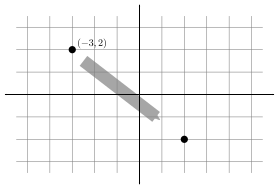
\includegraphics{transEg1.pdf}
\end{image}
Here is how you do it:
\begin{align*}
\mat{T}_{(5,-4)} \vec{p} &= 
\begin{bmatrix}
1 & 0 & 5 \\ 
0 & 1 & -4 \\
0 & 0 & 1
\end{bmatrix}
\begin{bmatrix}
-3 \\
2 \\
1
\end{bmatrix}\\
&=
\begin{bmatrix}
-3 + 0 + 5\\
0 + 2 - 4 \\
0 + 0 + 1
\end{bmatrix}\\
&=
\begin{bmatrix}
2\\
-2 \\
1
\end{bmatrix}
\end{align*}
Hence, we end up with the point $(2,-2)$. But you knew that already,
didn't you?
\end{example}

\begin{question} 
Can you demonstrate with algebra why translations are isometries?
\end{question}



\begin{question} 
We know how to translate individual points. How do we move entire
figures and other funky shapes?
\end{question}


\end{document}
